\chapter{Implementation}

\section{Codebase Design}

\subsection{Repository Overview}

\subsection{Site Navigation}

\section{Backend Development}

The following section details the backend's structure and development process. The final class structure is shown in Figure 3.1.

\begin{figure}[H]
    \centering
    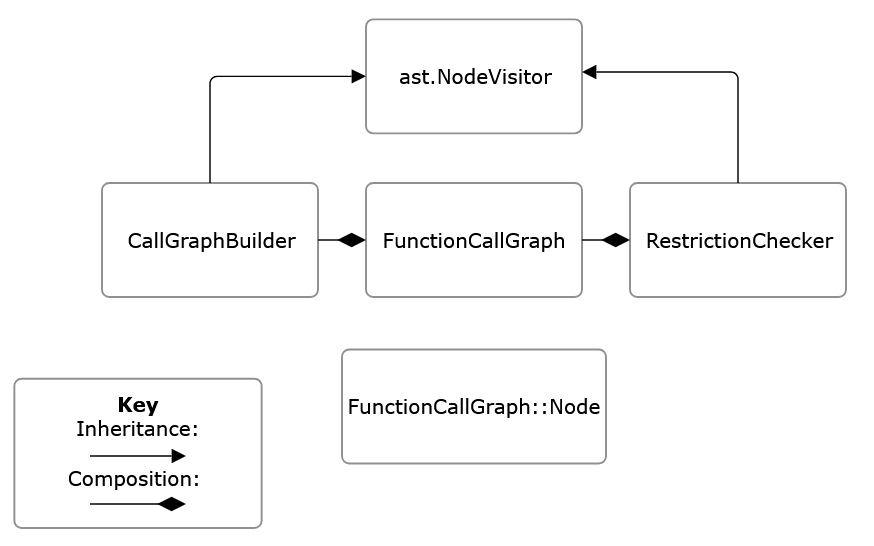
\includegraphics[width=0.75\linewidth]{implementation/backend-UML.png}
    \caption{UML for the backend's class structure.}
    \label{fig:placeholder}
\end{figure}

\subsection{RestrictionChecker}

This was the most fundamental aspect of the project, and thus the first piece of backend work completed. 
From the preparation work, it was decided that using the Python ast module would be the most reasonable approach.

\codeword{RestrictionChecker} inherits from the class \codeword{ast.NodeVisitor}, which traverses abstract syntax trees created by \codeword{ast.parse()}. By overriding the method \codeword{generic_visit()}, it checks for restrictions in four ways. First are restrictions that can be identified by the node's type. For example, an if statement's node will be of type \codeword{If}. On finding a node of this type, the checker knows it has found a restriction. Second, datatypes...
Third, recursion, which presented the most interesting challenge.
Finally, else statements need to be handled differently, since they do not have a node type. Instead, on identifying an if statement, separate checks discover whether the \codeword{orelse} attribute is populated.